\documentclass[10pt,twocolumn,letterpaper]{article}

\usepackage{iccv}

%------------------------------------------------------------------------------
%------------------------------------------------------------------------------
% hack for CVPR/ICCV style
\makeatletter
\@namedef{ver@everyshi.sty}{}
\makeatother

%------------------------------------------------------------------------------
% main packages
\usepackage[dvipsnames,svgnames,x11names]{xcolor}
\usepackage{tikz}
\usetikzlibrary{arrows.meta,shapes,calc,matrix,fit,positioning,backgrounds,decorations.markings,fadings}
\usepackage{pgfplots}
\usepackage{pgfplotstable}
\pgfplotsset{compat=1.9}
\usepackage{xstring}

%------------------------------------------------------------------------------
% externalization: requires defining \finalcopy first

\usepgfplotslibrary{external}
% \tikzexternalize[prefix=fig/extern/]
\newcommand{\extfig}[2]{\tikzsetnextfilename{#1}{#2}}
\newcommand{\noextfig}[1]{\tikzset{external/export next={false}}{#1}}
\newcommand{\extdata}[1]{\input{#1}}
\IfBeginWith*{\jobname}{fig/extern/}{\finalcopy}{}

%-----------------------------------------------------------------------------
% tikz styles

\tikzstyle{every picture}+=[
	remember picture,
	every text node part/.style={align=center},
	every matrix/.append style={ampersand replacement=\&},
]
\tikzstyle{tight} = [inner sep=0pt,outer sep=0pt]
\tikzstyle{node}  = [draw,circle,tight,minimum size=12pt,anchor=center]
\tikzstyle{op}    = [draw,circle,tight]
\tikzstyle{dot}   = [fill,draw,circle,inner sep=1pt,outer sep=0]
\tikzstyle{pt}    = [fill,draw,circle,inner sep=1.5pt,outer sep=.2pt]
\tikzstyle{box}   = [draw,thick,rectangle,inner sep=3pt]
\tikzstyle{high}  = [black!60]
\tikzstyle{group} = [high,box,opacity=.5]
\tikzstyle{dim1}  = [fill opacity=.3,text opacity=1]
\tikzstyle{dim2}  = [fill opacity=.5,text opacity=1]
\tikzstyle{dim3}  = [fill opacity=.7,text opacity=1]
\tikzstyle{rectc} = [tight,transform shape]
\tikzstyle{rect}  = [rectc,anchor=south west]

%-----------------------------------------------------------------------------
% framed figures

\newcommand{\framed}[3][1]{\extfig{#2}{\tikz{
	\node[tight](a){\fig[#1]{#3}};
	\node[tight,draw=gray,fit=(a)]{};
}}}

%-----------------------------------------------------------------------------
% pgfplots general options

\newcommand{\leg}[1]{\addlegendentry{#1}}

\tikzset{every mark/.append style={solid}}
\pgfplotsset{%smooth,
	grid=both, width=\columnwidth, try min ticks=5,
	every axis/.append style={font=\small},
	every axis plot/.append style={thick,mark=none,mark size=1.8,tension=0.18},
	legend cell align=left, legend style={fill opacity=0.8},
	xticklabel={\pgfmathprintnumber[assume math mode=true]{\tick}},
	yticklabel={\pgfmathprintnumber[assume math mode=true]{\tick}},
	nodes near coords math/.style={
		nodes near coords={\pgfmathprintnumber[assume math mode=true]{\pgfplotspointmeta}},
	},
}

\pgfplotsset{
	dash/.style={mark=o,dashed,opacity=0.6},
	dott/.style={mark=o,dotted,opacity=0.6},
	nolim/.style={enlargelimits=false},
	plain/.style={every axis plot/.append style={},nolim,grid=none},
}
\newcommand{\kilo}[1]{\thisrow{#1}/1000}

%--------------------------------------------------------------------

% layers
\pgfdeclarelayer{bg4}
\pgfdeclarelayer{bg3}
\pgfdeclarelayer{bg2}
\pgfdeclarelayer{bg1}
\pgfdeclarelayer{fg1}
\pgfdeclarelayer{fg2}
\pgfdeclarelayer{fg3}
\pgfdeclarelayer{fg4}
\pgfsetlayers{bg4,bg3,bg2,bg1,main,fg1,fg2,fg3,fg4}

%------------------------------------------------------------------------------
% 3d drawing

\pgfkeys{/tikz/.cd, aspect/.store in=\aspect, aspect=1}
\pgfkeys{/tikz/.cd, depth/.store in=\depth, depth=.5}
\pgfkeys{/tikz/.cd, stepx/.store in=\step, stepx=1}

\tikzstyle{geom} = [line join=bevel,aspect=1,depth=.5,z={(\depth*\aspect,\depth)}]
\tikzstyle{wire} = [geom,draw,thick]

% 3d coordinates
\def\cx[#1,#2,#3]{#1}
\def\cy[#1,#2,#3]{#2}
\def\cz[#1,#2,#3]{#3}
\def\ex[#1,#2,#3]{#1,0,0}
\def\ey[#1,#2,#3]{0,#2,0}
\def\ez[#1,#2,#3]{0,0,#3}

% lines along x, y, or z
\newcommand{\zline}[3][]{%
\path[geom,#1] #2 -- +(\cx[#3],\cy[#3]);
}
\newcommand{\yline}[3][]{%
\path[geom,#1,shift={#2},xslant=\aspect]
	(0,0) -- +(\cx[#3],\depth*\cz[#3]);
}
\newcommand{\xline}[3][]{%
\path[geom,#1,shift={#2},yslant=1/\aspect]
	(0,0) -- +(\aspect*\depth*\cz[#3],\cy[#3]);
}

% rectangles / grids along x, y, or z
\newcommand{\zrect}[3][]{%
\path[geom,#1] #2 rectangle +(\cx[#3],\cy[#3]);
}
\newcommand{\yrect}[3][]{%
\path[geom,#1,shift={#2},xslant=\aspect]
	(0,0) rectangle +(\cx[#3],\depth*\cz[#3]);
}
\newcommand{\xrect}[3][]{%
\path[geom,#1,shift={#2},yslant=1/\aspect]
	(0,0) rectangle +(\aspect*\depth*\cz[#3],\cy[#3]);
}
\newcommand{\xgrid}[3][]{%
\path[geom,#1,shift={#2},yslant=1/\aspect,xstep=\aspect*\depth*\step]
	(0,0) grid +(\aspect*\depth*\cz[#3],\cy[#3]);
}

% parallepiped
\newcommand{\para}[4][]{%
\zrect[#1]{(#3)}{#4}                 % front
\yrect[#1]{($(#3)+(\ey[#4])$)}{#4}   % top
\xrect[#1]{($(#3)+(\ex[#4])$)}{#4}   % right
\path[geom]
	(#3) coordinate(#2-southwest)
	($(#3)+(#4)$) coordinate(#2-northeast)
	($(#3)+(\ey[#4])$) coordinate(#2-northwest)
	($(#3)+(#4)-(\ey[#4])$) coordinate(#2-southeast)
	($(#3)+.5*(\ex[#4])$) coordinate(#2-south)
	($(#3)+(#4)-.5*(\ex[#4])$) coordinate(#2-north)
	($(#3)+.5*(\ex[#4])+.5*(#4)$) coordinate(#2-center)
	(#2-southwest |- #2-center) coordinate(#2-west)
	(#2-center -| #2-northeast) coordinate(#2-east)
	;
}

%------------------------------------------------------------------------------
% space before \paragraph (default 4.05ex)
\makeatletter
\renewcommand\paragraph{\@startsection{paragraph}{4}{\z@}{1ex}{-1em}{\normalfont\normalsize\bfseries}}
\makeatother
%------------------------------------------------------------------------------

\usepackage{times}
\usepackage{epsfig}
\usepackage{graphicx}
\usepackage{amsmath}
\usepackage{amssymb}

\usepackage{times}
\usepackage{helvet}
\usepackage{courier}
\usepackage{url}
\usepackage{graphicx}
\usepackage{booktabs}
\usepackage{subcaption}
\usepackage{amsmath}
\usepackage{amsfonts}
\usepackage{mathtools}
\usepackage{multirow}
\usepackage{enumitem}

%
\usepackage{times}
\usepackage{epsfig}
\usepackage{graphicx}
\usepackage{amsmath}
\usepackage{amssymb}
\usepackage{tabularx}

\usepackage{verbatim}
\usepackage{multirow}
\usepackage{array}

\usepackage{amsthm}
\usepackage{xspace}
\usepackage[svgnames]{xcolor}

\usepackage{pifont}

\frenchspacing
\setlength{\pdfpagewidth}{8.5in}
\setlength{\pdfpageheight}{11in}

\usepackage[pagebackref=true,breaklinks=true,letterpaper=true,colorlinks,bookmarks=false]{hyperref}

\iccvfinalcopy

\def\httilde{\mbox{\tt\raisebox{-.5ex}{\symbol{126}}}}

\begin{document}

\title{All the attention you need:\\Global-local, spatial-channel attention for image retrieval}

\author{Chull Hwan Song\\
{\small Odd Concepts}
\and
Hye Joo Han\\
{\small Odd Concepts}
\and
Yannis Avrithis\\
{\small Inria, Univ Rennes, CNRS, IRISA}
}

\maketitle

% !TEX root = ../paper.tex

\newcommand{\head}[1]{{\smallskip\noindent\textbf{#1}}}
\newcommand{\alert}[1]{{\color{red}{#1}}}
\newcommand{\sm}{\scriptsize}
\newcommand{\eq}[1]{(\ref{eq:#1})}

% \newcommand{\Th}[1]{\tableheadline{#1}}
\newcommand{\Th}[1]{\textsc{#1}}
\newcommand{\mr}[2]{\multirow{#1}{*}{#2}}
\newcommand{\mc}[2]{\multicolumn{#1}{c}{#2}}
\newcommand{\mca}[3]{\multicolumn{#1}{#2}{#3}}
\newcommand{\tb}[1]{\textbf{#1}}
\newcommand{\ch}{\checkmark}

\newcommand{\red}[1]{{\color{red}{#1}}}
\newcommand{\blue}[1]{{\color{blue}{#1}}}
\newcommand{\green}[1]{\color{green}{#1}}
\newcommand{\gray}[1]{{\color{gray}{#1}}}

\newcommand{\citeme}[1]{\red{[XX]}}
\newcommand{\refme}[1]{\red{(XX)}}

\newcommand{\fig}[2][1]{\includegraphics[width=#1\linewidth]{fig/#2}}
\newcommand{\figh}[2][1]{\includegraphics[height=#1\linewidth]{fig/#2}}

%--------------------------------------------------------------------

\newcommand{\tran}{^\top}
\newcommand{\mtran}{^{-\top}}
\newcommand{\zcol}{\mathbf{0}}
\newcommand{\zrow}{\zcol\tran}

\newcommand{\ind}{\mathbbm{1}}
\newcommand{\expect}{\mathbb{E}}
\newcommand{\nat}{\mathbb{N}}
\newcommand{\zahl}{\mathbb{Z}}
\newcommand{\real}{\mathbb{R}}
\newcommand{\proj}{\mathbb{P}}
\newcommand{\prob}{\mathbf{Pr}}
\newcommand{\normal}{\mathcal{N}}

\newcommand{\mif}{\textrm{if}\ }
\newcommand{\other}{\textrm{otherwise}}
\newcommand{\minimize}{\textrm{minimize}\ }
\newcommand{\maximize}{\textrm{maximize}\ }
\newcommand{\st}{\textrm{subject\ to}\ }

\newcommand{\id}{\operatorname{id}}
\newcommand{\const}{\operatorname{const}}
\newcommand{\sgn}{\operatorname{sgn}}
\newcommand{\var}{\operatorname{Var}}
\newcommand{\mean}{\operatorname{mean}}
\newcommand{\trace}{\operatorname{tr}}
\newcommand{\diag}{\operatorname{diag}}
\newcommand{\vect}{\operatorname{vec}}
\newcommand{\cov}{\operatorname{cov}}
\newcommand{\sign}{\operatorname{sign}}
\newcommand{\prj}{\operatorname{proj}}

\newcommand{\sigmoid}{\operatorname{sigmoid}}
\newcommand{\softmax}{\operatorname{softmax}}
\newcommand{\clip}{\operatorname{clip}}

\newcommand{\defn}{\mathrel{:=}}
\newcommand{\peq}{\mathrel{+\!=}}
\newcommand{\meq}{\mathrel{-\!=}}

\newcommand{\floor}[1]{\left\lfloor{#1}\right\rfloor}
\newcommand{\ceil}[1]{\left\lceil{#1}\right\rceil}
\newcommand{\inner}[1]{\left\langle{#1}\right\rangle}
\newcommand{\norm}[1]{\left\|{#1}\right\|}
\newcommand{\abs}[1]{\left|{#1}\right|}
\newcommand{\frob}[1]{\norm{#1}_F}
\newcommand{\card}[1]{\left|{#1}\right|\xspace}
\newcommand{\diff}{\mathrm{d}}
\newcommand{\der}[3][]{\frac{d^{#1}#2}{d#3^{#1}}}
\newcommand{\pder}[3][]{\frac{\partial^{#1}{#2}}{\partial{#3^{#1}}}}
\newcommand{\ipder}[3][]{\partial^{#1}{#2}/\partial{#3^{#1}}}
\newcommand{\dder}[3]{\frac{\partial^2{#1}}{\partial{#2}\partial{#3}}}

\newcommand{\wb}[1]{\overline{#1}}
\newcommand{\wt}[1]{\widetilde{#1}}

\def\xssp{\hspace{1pt}}
\def\ssp{\hspace{3pt}}
\def\msp{\hspace{5pt}}
\def\lsp{\hspace{12pt}}

\newcommand{\cA}{\mathcal{A}}
\newcommand{\cB}{\mathcal{B}}
\newcommand{\cC}{\mathcal{C}}
\newcommand{\cD}{\mathcal{D}}
\newcommand{\cE}{\mathcal{E}}
\newcommand{\cF}{\mathcal{F}}
\newcommand{\cG}{\mathcal{G}}
\newcommand{\cH}{\mathcal{H}}
\newcommand{\cI}{\mathcal{I}}
\newcommand{\cJ}{\mathcal{J}}
\newcommand{\cK}{\mathcal{K}}
\newcommand{\cL}{\mathcal{L}}
\newcommand{\cM}{\mathcal{M}}
\newcommand{\cN}{\mathcal{N}}
\newcommand{\cO}{\mathcal{O}}
\newcommand{\cP}{\mathcal{P}}
\newcommand{\cQ}{\mathcal{Q}}
\newcommand{\cR}{\mathcal{R}}
\newcommand{\cS}{\mathcal{S}}
\newcommand{\cT}{\mathcal{T}}
\newcommand{\cU}{\mathcal{U}}
\newcommand{\cV}{\mathcal{V}}
\newcommand{\cW}{\mathcal{W}}
\newcommand{\cX}{\mathcal{X}}
\newcommand{\cY}{\mathcal{Y}}
\newcommand{\cZ}{\mathcal{Z}}

\newcommand{\vA}{\mathbf{A}}
\newcommand{\vB}{\mathbf{B}}
\newcommand{\vC}{\mathbf{C}}
\newcommand{\vD}{\mathbf{D}}
\newcommand{\vE}{\mathbf{E}}
\newcommand{\vF}{\mathbf{F}}
\newcommand{\vG}{\mathbf{G}}
\newcommand{\vH}{\mathbf{H}}
\newcommand{\vI}{\mathbf{I}}
\newcommand{\vJ}{\mathbf{J}}
\newcommand{\vK}{\mathbf{K}}
\newcommand{\vL}{\mathbf{L}}
\newcommand{\vM}{\mathbf{M}}
\newcommand{\vN}{\mathbf{N}}
\newcommand{\vO}{\mathbf{O}}
\newcommand{\vP}{\mathbf{P}}
\newcommand{\vQ}{\mathbf{Q}}
\newcommand{\vR}{\mathbf{R}}
\newcommand{\vS}{\mathbf{S}}
\newcommand{\vT}{\mathbf{T}}
\newcommand{\vU}{\mathbf{U}}
\newcommand{\vV}{\mathbf{V}}
\newcommand{\vW}{\mathbf{W}}
\newcommand{\vX}{\mathbf{X}}
\newcommand{\vY}{\mathbf{Y}}
\newcommand{\vZ}{\mathbf{Z}}

\newcommand{\va}{\mathbf{a}}
\newcommand{\vb}{\mathbf{b}}
\newcommand{\vc}{\mathbf{c}}
\newcommand{\vd}{\mathbf{d}}
\newcommand{\ve}{\mathbf{e}}
\newcommand{\vf}{\mathbf{f}}
\newcommand{\vg}{\mathbf{g}}
\newcommand{\vh}{\mathbf{h}}
\newcommand{\vi}{\mathbf{i}}
\newcommand{\vj}{\mathbf{j}}
\newcommand{\vk}{\mathbf{k}}
\newcommand{\vl}{\mathbf{l}}
\newcommand{\vm}{\mathbf{m}}
\newcommand{\vn}{\mathbf{n}}
\newcommand{\vo}{\mathbf{o}}
\newcommand{\vp}{\mathbf{p}}
\newcommand{\vq}{\mathbf{q}}
\newcommand{\vr}{\mathbf{r}}
\newcommand{\Vs}{\mathbf{s}}
\newcommand{\vt}{\mathbf{t}}
\newcommand{\vu}{\mathbf{u}}
\newcommand{\vv}{\mathbf{v}}
\newcommand{\vw}{\mathbf{w}}
\newcommand{\vx}{\mathbf{x}}
\newcommand{\vy}{\mathbf{y}}
\newcommand{\vz}{\mathbf{z}}

\newcommand{\vone}{\mathbf{1}}
\newcommand{\vzero}{\mathbf{0}}

\newcommand{\valpha}{{\boldsymbol{\alpha}}}
\newcommand{\vbeta}{{\boldsymbol{\beta}}}
\newcommand{\vgamma}{{\boldsymbol{\gamma}}}
\newcommand{\vdelta}{{\boldsymbol{\delta}}}
\newcommand{\vepsilon}{{\boldsymbol{\epsilon}}}
\newcommand{\vzeta}{{\boldsymbol{\zeta}}}
\newcommand{\veta}{{\boldsymbol{\eta}}}
\newcommand{\vtheta}{{\boldsymbol{\theta}}}
\newcommand{\viota}{{\boldsymbol{\iota}}}
\newcommand{\vkappa}{{\boldsymbol{\kappa}}}
\newcommand{\vlambda}{{\boldsymbol{\lambda}}}
\newcommand{\vmu}{{\boldsymbol{\mu}}}
\newcommand{\vnu}{{\boldsymbol{\nu}}}
\newcommand{\vxi}{{\boldsymbol{\xi}}}
\newcommand{\vomikron}{{\boldsymbol{\omikron}}}
\newcommand{\vpi}{{\boldsymbol{\pi}}}
\newcommand{\vrho}{{\boldsymbol{\rho}}}
\newcommand{\vsigma}{{\boldsymbol{\sigma}}}
\newcommand{\vtau}{{\boldsymbol{\tau}}}
\newcommand{\vupsilon}{{\boldsymbol{\upsilon}}}
\newcommand{\vphi}{{\boldsymbol{\phi}}}
\newcommand{\vchi}{{\boldsymbol{\chi}}}
\newcommand{\vpsi}{{\boldsymbol{\psi}}}
\newcommand{\vomega}{{\boldsymbol{\omega}}}

\newcommand{\rLambda}{\mathrm{\Lambda}}
\newcommand{\rSigma}{\mathrm{\Sigma}}

\newcommand{\vLambda}{\bm{\rLambda}}
\newcommand{\vSigma}{\bm{\rSigma}}

% big cdot
\makeatletter
\newcommand*\bdot{\mathpalette\bdot@{.7}}
\newcommand*\bdot@[2]{\mathbin{\vcenter{\hbox{\scalebox{#2}{$\m@th#1\bullet$}}}}}
\makeatother

%--------------------------------------------------------------------
% Add a period to the end of an abbreviation unless there's one
% already, then \xspace.
\makeatletter
\DeclareRobustCommand\onedot{\futurelet\@let@token\@onedot}
\def\@onedot{\ifx\@let@token.\else.\null\fi\xspace}

\def\eg{\emph{e.g}\onedot} \def\Eg{\emph{E.g}\onedot}
\def\ie{\emph{i.e}\onedot} \def\Ie{\emph{I.e}\onedot}
\def\cf{\emph{cf}\onedot} \def\Cf{\emph{Cf}\onedot}
\def\etc{\emph{etc}\onedot} \def\vs{\emph{vs}\onedot}
\def\wrt{w.r.t\onedot} \def\dof{d.o.f\onedot} \def\aka{a.k.a\onedot}
\def\etal{\emph{et al}\onedot}
\makeatother

%------------------------------------------------------------------------------
% method shortcuts

\def\vlad{VLAD\xspace}
\def\smk{SMK$^{\star}$\xspace}
\def\asmk{ASMK$^{\star}$\xspace}
\def\sp{SP\xspace}
\def\qe{QE\xspace}
\def\hqe{HQE\xspace}
\def\dfs{DFS\xspace}
\def\off{O}
\def\hesaff{HesAff\xspace}
\def\rsift{rSIFT\xspace}
\def\delf{DELF\xspace}

%------------------------------------------------------------------------------
% data shortcuts

\def\oxf5k{Ox5k\xspace}
\def\paris6k{Par6k\xspace}

\def\roxf{$\mathcal{R}$Oxford}
\def\rox{$\mathcal{R}$Oxf}
\def\ro{$\mathcal{R}$O}
\def\rpar{$\mathcal{R}$Paris}
\def\rpa{$\mathcal{R}$Par}
\def\rp{$\mathcal{R}$Pe}
\def\r1m{$\mathcal{R}$1M}
\def\rs{$\mathcal{R}$100k}

%------------------------------------------------------------------------------
% colors

\definecolor{greenn}{rgb}{0.30,0.69,0.31}
\definecolor{redd}{rgb}{0.3,0.2,0.7}
\definecolor{red}{rgb}{0.8,0.1,0.1}

\newcommand{\ok}[1]{\color{redd}{#1}}
\newcommand{\okg}[1]{\color{greenn}{#1}}


\begin{abstract}
We address representation learning for large-scale instance-level image retrieval. Apart from backbone, training pipelines and loss functions, popular approaches have focused on different spatial pooling and attention mechanisms, which are at the core of learning a powerful global image representation. There are different forms of attention according to the interaction of elements of the feature tensor (local and global) and the dimensions where it is applied (spatial and channel). Unfortunately, each study addresses only one or two forms of attention and applies it to different problems like classification, detection or retrieval.

We present \emph{global-local attention module} (GLAM), which is attached at the end of a backbone network and incorporates all four forms of attention: local and global, spatial and channel. We obtain a new feature tensor and, by spatial pooling, we learn a powerful embedding for image retrieval.
Focusing on global descriptors, we provide empirical evidence of the interaction of all forms of attention and improve the state of the art on standard benchmarks.
\end{abstract}

%auto-ignore
\section{Introduction}


Language model pre-training has been shown to be effective for improving many natural language processing tasks~\cite{dai-le:2015:_semi, peters-etal:2018:_deep, radford-etal:2018, howard-ruder:2018}. These include sentence-level tasks such as natural language inference~\cite{bowman-etal:2015, williams-nangia-bowman:2018} and paraphrasing~\cite{dolan-brockett:2005:_autom}, which aim to predict the relationships between sentences by analyzing them holistically, as well as token-level tasks such as named entity recognition and question answering, where models are required to produce fine-grained output at the token level~\cite{tjong-de:2003, rajpurkar-etal:2016:_squad}.


There are two existing strategies for applying pre-trained language representations to downstream tasks: {\em feature-based} and {\em fine-tuning}. The feature-based approach, such as ELMo~\cite{peters-etal:2018:_deep}, uses task-specific architectures that include the pre-trained representations as additional features. The fine-tuning approach, such as the Generative Pre-trained Transformer (OpenAI GPT)~\cite{radford-etal:2018}, introduces minimal task-specific parameters, and is trained on the downstream tasks by simply fine-tuning {\em all} pre-trained parameters. The two approaches share the same objective function during pre-training, where they use unidirectional language models to learn general language representations.

We argue that current techniques restrict the power of the pre-trained representations, especially for the fine-tuning approaches. The major limitation is that standard language models are unidirectional, and this limits the choice of architectures that can be used during pre-training. For example, in OpenAI GPT, the authors use a left-to-right architecture, where every token can only attend to previous tokens in the self-attention layers of the Transformer~\cite{vaswani-etal:2017:_atten}. Such restrictions are sub-optimal for sentence-level tasks, and could be very harmful when applying fine-tuning based approaches to token-level tasks such as  question answering, where it is crucial to incorporate context from both directions.

In this paper, we improve the fine-tuning based approaches by proposing \bert: \textbf{B}idirectional \textbf{E}ncoder \textbf{R}epresentations from \textbf{T}ransformers. \bert alleviates the previously mentioned unidirectionality constraint by using a ``masked language model''~(MLM) pre-training objective, inspired by the Cloze task~\cite{taylor:1953:_cloze}. The masked language model randomly masks some of the tokens from the input, and the objective is to predict the original vocabulary id of the masked word based only on its context. Unlike left-to-right language model pre-training, the MLM objective enables the representation to fuse the left and the right context, which allows us to pre-train a deep bidirectional Transformer. In addition to the masked language model, we also use a ``next sentence prediction'' task that jointly pre-trains text-pair representations. The contributions of our paper are as follows:
\begin{itemize}[leftmargin=1em]
  \item We demonstrate the importance of bidirectional pre-training for language representations. Unlike \citet{radford-etal:2018}, which uses unidirectional language models for pre-training, \bert uses masked language models to enable pre-trained deep bidirectional representations. This is also in contrast to \citet{peters-etal:2018:_deep}, which uses a shallow concatenation of independently trained left-to-right and right-to-left LMs.
  \item We show that pre-trained representations reduce the need for many heavily-engineered task-specific architectures. \bert is the first fine-tuning based representation model that achieves state-of-the-art performance on a large suite of sentence-level {\em and} token-level tasks, outperforming many task-specific architectures.
  \item \bert advances the state of the art for eleven NLP tasks. 
%
    The code and pre-trained models are available at \url{https://github.com/google-research/bert}.
\end{itemize}

%auto-ignore

\section{Related Work}
There is a long history of pre-training general language representations, and we briefly review the most widely-used approaches in this section.


\subsection{Unsupervised Feature-based Approaches}
Learning widely applicable representations of words has been an active area of research for decades, including non-neural~\cite{brown-etal:1992:_class, ando-zhang:2005, blitzer-mcdonald-pereira:2006:_domain} and neural~\cite{mikolov-etal:2013, pennington-socher-manning:2014:_glove} methods. Pre-trained word embeddings are an integral part of modern NLP systems, offering significant improvements over embeddings learned from scratch~\cite{turian-ratinov-bengio:2010:_word_repres}. To pre-train word embedding vectors, left-to-right language modeling objectives have been used~\cite{minh09}, as well as objectives to  discriminate correct from incorrect words in left and right context~\cite{mikolov-etal:2013}.

These approaches have been generalized to coarser granularities, such as sentence embeddings~\cite{kiros-etal:2015:_skip, logeswaran2018an} or paragraph embeddings~\cite{le-mikolov:2014:_distr}. To train sentence representations, prior work has used objectives to rank candidate next sentences  \cite{DBLP:journals/corr/JerniteBS17, logeswaran2018an},  left-to-right generation of next sentence words given a representation of the previous sentence~\cite{kiros-etal:2015:_skip}, or denoising auto-encoder derived objectives~\cite{hill16}.

%
\begin{figure*}[t!]
%\small
\begin{center}
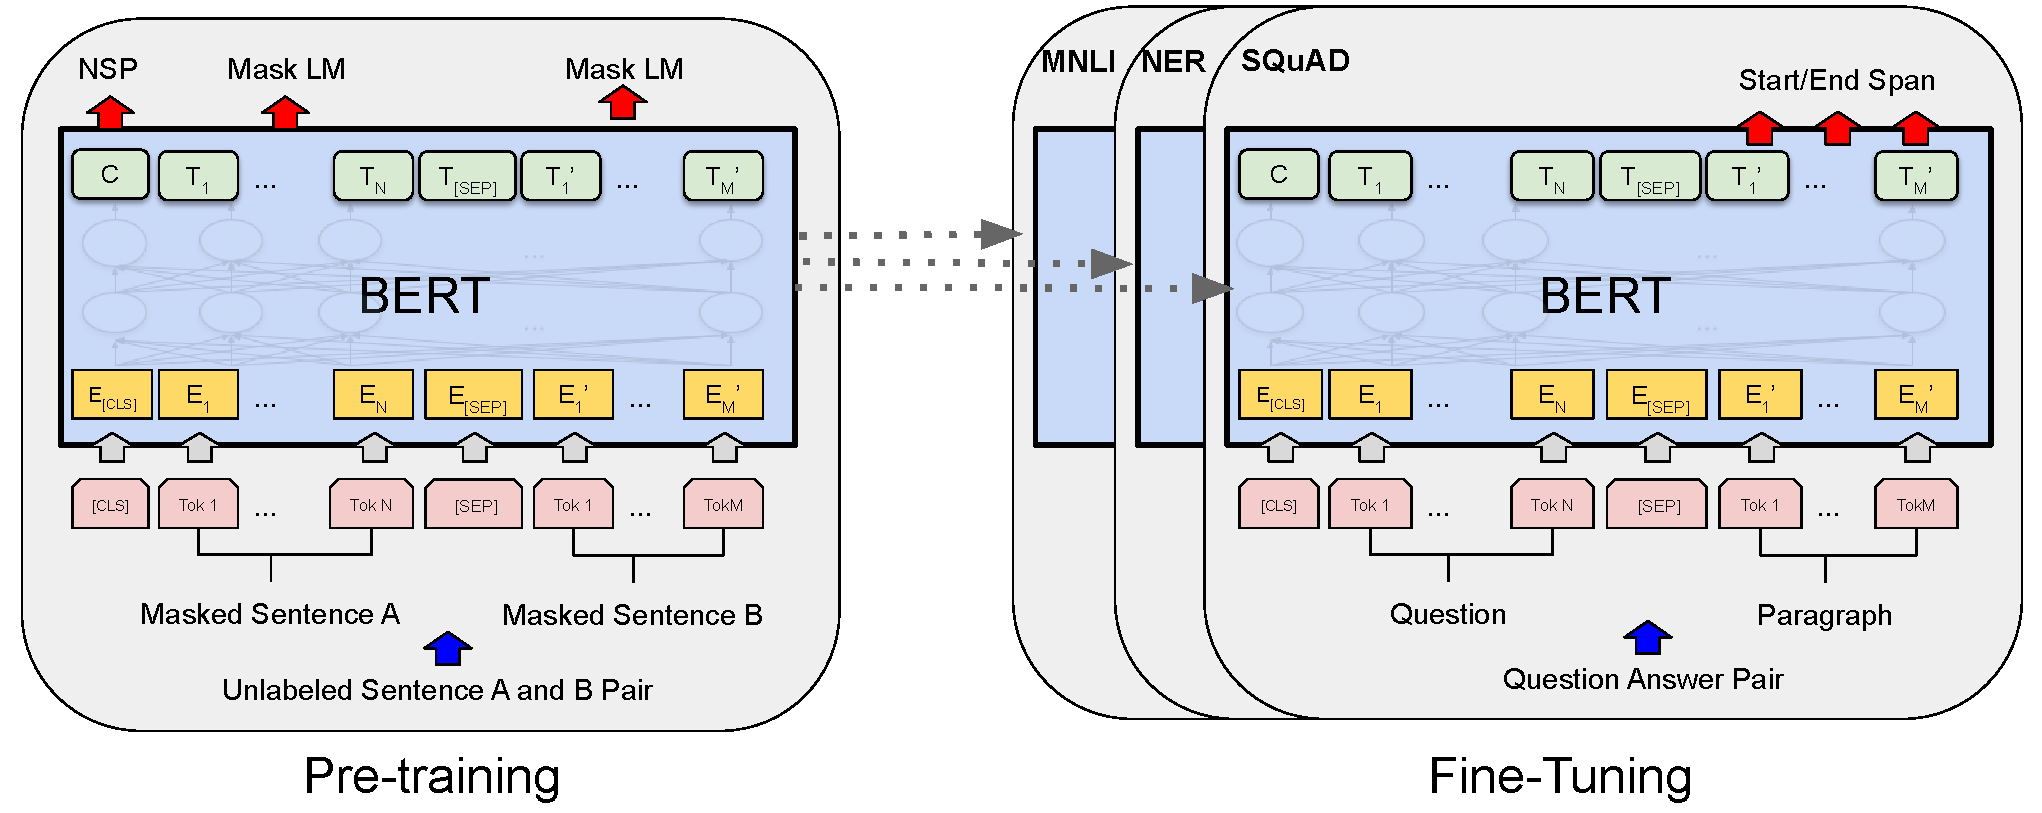
\includegraphics[width=1\textwidth]{BERT_Overall.pdf}
\end{center}
\caption{Overall pre-training and fine-tuning procedures for BERT. Apart from output layers, the same architectures are used in both pre-training and fine-tuning. The same pre-trained model parameters are used to initialize models for different down-stream tasks.  During fine-tuning, all parameters are fine-tuned. {\tt [CLS]} is a special symbol added
in front of every input example, and {\tt [SEP]} is a special separator token (e.g. separating  questions/answers).}
\label{fig:bert_overall}
\end{figure*}
%



ELMo and its predecessor~\cite{peters-etal:2017:_semi, peters-etal:2018:_deep} generalize traditional word embedding research along a different dimension. They extract \emph{context-sensitive} features from a left-to-right and a right-to-left language model. The contextual representation of each token is the concatenation of the left-to-right and right-to-left representations. When integrating contextual word embeddings with existing task-specific architectures, ELMo advances the state of the art for several major NLP benchmarks~\cite{peters-etal:2018:_deep} including question answering~\cite{rajpurkar-etal:2016:_squad}, sentiment analysis~\cite{socher-etal:2013:_recur}, and named entity recognition~\cite{tjong-de:2003}.
\citet{melamud2016context2vec} proposed learning contextual representations through a task to predict a single word from both left and right context
using LSTMs. Similar to ELMo, their model is feature-based and not deeply bidirectional. 
\citet{fedus2018maskgan} shows that the cloze task can be used to improve the robustness of text generation models. 




\subsection{Unsupervised Fine-tuning Approaches}

As with the feature-based approaches, the first works in this direction only pre-trained word embedding parameters from unlabeled text ~\cite{collobert-weston:2008}.  

More recently, sentence or document encoders which produce contextual token representations have been pre-trained from unlabeled text and fine-tuned for a supervised downstream task~\cite{dai-le:2015:_semi, howard-ruder:2018, radford-etal:2018}.  The advantage of these approaches is that few parameters need to be learned from scratch. At least partly due to this advantage, OpenAI GPT~\cite{radford-etal:2018} achieved previously state-of-the-art results on many sentence-level tasks from the GLUE benchmark~\cite{wang-etal:2018:_glue}.  Left-to-right language modeling and auto-encoder objectives have been used for pre-training such models~\cite{howard-ruder:2018, radford-etal:2018,dai-le:2015:_semi}.





\subsection{Transfer Learning from Supervised Data}

There has also been work showing effective transfer from supervised tasks with large datasets, such as natural language inference~\cite{conneau-EtAl:2017:EMNLP2017} and machine translation~\cite{mccann-etal:2017:_learn_trans}. 
Computer vision research has also demonstrated the importance of transfer learning from large pre-trained models, where an effective recipe is to fine-tune models pre-trained with ImageNet~\cite{imagenet_cvpr09, yosinski2014transferable}. 




\section{\model{}: Synergizing \texttt{Re}asoning + \texttt{Act}ing}
\label{sec:react}








Consider a general setup of an agent interacting with an environment for task solving. At time step $t$, an agent receives an observation $o_t \in \mathcal{O}$ from the environment and takes an action $a_t \in \mathcal{A}$ following some policy $\pi(a_t | c_t)$, where $c_t = (o_1, a_1, \cdots, o_{t-1}, a_{t-1}, o_t)$ is the \textit{context} to the agent. Learning a policy is challenging when the mapping $c_t \mapsto a_t$ is highly implicit and requires extensive computation. 
For example, the agent shown in Figure~\ref{fig:teaser}(1c) is unable to generate the correct final action (Act 4) to finish the QA task as it requires complex reasoning over the trajectory context (Question, Act 1-3, Obs 1-3).
Similarly, the agent shown in Figure~\ref{fig:teaser}(2a) fails to comprehend from the context that sinkbasin 1 does not contain peppershaker 1, thus keep producing hallucinating actions.


The idea of \model{} is simple: we augment the agent's action space to $\mathcal{\hat{A}} = \mathcal{A} \cup \mathcal{L}$, where $\mathcal{L}$ is the space of language. An action $\hat{a}_t \in \mathcal{L}$ in the language space, which we will refer to as a \textit{thought} or a \textit{reasoning trace}, does not affect the external environment, thus leading to no observation feedback. Instead, a thought $\hat{a}_t$ aims to compose useful information by reasoning over the current context $c_t$, and update the context $c_{t+1} = (c_t, \hat{a}_t)$ to support future reasoning or acting. 
As shown in Figure~\ref{fig:teaser}, there could be various types of useful thoughts, e.g.\,decomposing task goals and create action plans (2b, Act 1; 1d, Thought 1), injecting commonsense knowledge relevant to task solving (2b, Act 1), extracting important parts from observations (1d, Thought2, 4), track progress and transit action plans (2b, Act 8), handle exceptions and adjust action plans (1d, Thought 3), and so on. 


However, as the language space $\mathcal{L}$ is unlimited, learning in this augmented action space is difficult and requires strong language priors. In this paper, we mainly focus on 
the setup where a frozen large language model, PaLM-540B~\citep{chowdhery2022palm}\footnote{We show some GPT-3~\citep{brown2020language} results in Appendix~\ref{sec:gpt3}, which outperforms PaLM-540B. }, is prompted with few-shot in-context examples to generate both domain-specific actions and free-form language thoughts for task solving (Figure~\ref{fig:teaser} (1d), (2b)). Each in-context example is a human trajectory of actions, thoughts, and environment observations to solve a task instance (see Appendix~\ref{sec:prompts}). 
For the tasks where reasoning is of primary importance (Figure~\ref{fig:teaser}(1)), we alternate the generation of thoughts and actions so that the task-solving trajectory consists of multiple thought-action-observation steps.
In contrast, for  decision making tasks that potentially involve a large number of actions (Figure~\ref{fig:teaser}(2)), thoughts only need to appear sparsely in the most relevant positions of a trajectory, so we let the language model decide the asynchronous occurrence of thoughts and actions for itself.

Since decision making and reasoning capabilities are integrated into a large language model, \model{} enjoys several unique features:
    \textbf{A) Intuitive and easy to design}: Designing \model{} prompts is straightforward as human annotators just type down their thoughts in language on top of their actions taken. No ad-hoc format choice, thought design, or example selection is used in this paper. We detail prompt design for each task in Sections~\ref{sec:knowledge} and \ref{decision_making_tasks}.
    \textbf{B) General and flexible}: Due to the flexible thought space and thought-action occurrence format, \model{} works for diverse tasks with distinct action spaces and reasoning needs, including but not limited to QA, fact verification, text game, and web navigation.
    \textbf{C) Performant and robust}: \model{} shows strong generalization to new task instances while learning solely from one to six in-context examples, consistently outperforming baselines with only reasoning or acting across different domains. We also show in Section~\ref{sec:knowledge} additional benefits when finetuning is enabled, and in Section~\ref{decision_making_tasks} how \model{} performance is robust to prompt selections.
    \textbf{D) Human aligned and controllable}: \model{} promises an interpretable sequential decision making and reasoning process where humans can easily inspect reasoning and factual correctness. Moreover, humans can also control or correct the agent behavior on the go by thought editing, as shown in Figure~\ref{fig:edit} in Section~\ref{decision_making_tasks}.
































\section{Experiments}
\label{sec:exp}

%------------------------------------------------------------------------------
\begin{figure*}
\centering
\fig{10_2}
\caption{Examples of our ranking results. In each row, the first image on the left (pink dotted outline) is a query image with a target object (red crop box), and the following are the top ranking images for the query. Orange solid outline: positive images for the query; red solid outline: negative.}
\label{fig:fig8}
\end{figure*}
%------------------------------------------------------------------------------

\subsection{Datasets}

\paragraph{Training set}

There are a number of open landmark datasets commonly used for training in image retrieval studies, including \emph{neural code} (NC)~\cite{Babenko01}, \emph{neural code clean} (NC-clean)~\cite{Gordo01}, as well as Google Landmarks v1 (GLDv1)~\cite{Noh01} and v2 (GLDv2)~\cite{Weyand01}. \autoref{tab:table1} shows relevant statistics. These datasets can be categorized into noisy and clean. The clean sets were obtained from the original noisy sets for more effective training~\cite{Gordo01, Weyand01}. The original noisy datasets are much larger, but they have high intra-class variability. Each class can include visually dissimilar images such as exterior and interior views of a building or landmark, including floor plans and paintings inside. The clean datasets focus on views directly relevant to landmark recognition but have a much smaller number of images.

%------------------------------------------------------------------------------

\paragraph{Evaluation set and metrics}

We use four common evaluation datasets for landmark image retrieval: Oxford5k (\oxf5k)~\cite{Philbin01}, Paris6k (\paris6k)~\cite{Philbin02}, as well as Revisited Oxford (\roxf~or \rox) and Paris (\rpar~or \rpa)~\cite{RITAC18}. \roxf~and \rpar~are used with and without one million distractors (\r1m)~\cite{Ng01} and evaluated using the Medium and Hard protocols~\cite{RITAC18}. We evaluate using \emph{mean Average Precision} (mAP) and \emph{mean precision at} 10 (mP@10).

%------------------------------------------------------------------------------

\subsection{Implementation details}

We train on 8 TITAN RTX 2080Ti GPUs. All models are pre-trained on ImageNet~\cite{Russakovsky01} and implemented in PyTorch \cite{Paszke01}. For fair comparisons, we set a training environment similar to the those  of compared studies~\cite{Yokoo01, Weyand01, Ng01, RITAC18}. We employ ResNet101~\cite{Zhang01} as a backbone model. The kernel size $k$ of ECANet in \autoref{sec:local} is set to 3. The parameter $p$ of GeM in \autoref{sec:embed} is set to 3 and the dimension $d$ of final embeddings to 512. We adopt ArcFace~\cite{Deng01}, a cosine-softmax based loss, with a margin of 0.3. We use stochastic gradient descent with initial learning rate $10^{-3}$, momentum 0.9 and weight decay $10^{-5}$.

We adopt the batch sampling of Yokoo \etal~\cite{Yokoo01} where mini-batch samples with similar aspect ratios are resized to a particular size. Here, we use a batch size of 64. For image augmentation, we apply scaling, random cropping, and varied illumination. At inference, we apply a multi-resolution representation~\cite{Gordo01} to query and database images.

Our method is denoted as GLAM (\emph{global-local attention module}). Using the backbone model alone is referred to as \emph{baseline}. It is compatible with recent models based on ResNet101-GeM trained with ArcFace~\cite{Weyand01, Ng01}. Adding our local attention (\autoref{sec:local}) to the baseline model is denoted \emph{+local}, while adding our global attention (\autoref{sec:global}) is denoted \emph{+global}. Since we focus on representation learning, we do not consider post-processing methods like geometry-based re-ranking \cite{Noh01, simeoni2019local, Weyand01} or graph-based re-ranking~\cite{Donoser01, iscen2017efficient, Yang01}.

%------------------------------------------------------------------------------
\begin{table}
\centering
\small
\begin{tabular}{lcc} \toprule
\Th{Train Set} & \Th{\#Images} & \Th{\#Classes} \\ \midrule
NC-noisy &  213,678 & 672 \\
NC-clean & 27,965 & 581 \\
SfM-120k & 117,369 & 713 \\
GLDv1-noisy & 1,225,029  &  14, 951 \\
GLDv2-noisy & 4,132,914  &  203,094 \\
GLDv2-clean & 1,580,470 & 81,313 \\
\bottomrule
\end{tabular}
\caption{Statistics of different training sets.}
\label{tab:table1}
\end{table}
%------------------------------------------------------------------------------


\subsection{Benchmarking}
\label{sec:SOTA}

%------------------------------------------------------------------------------
\begin{table}
\centering
\scriptsize
\setlength{\tabcolsep}{0.6pt}
\begin{tabular}{l*{8}{c}} \toprule
\mr{2}{\Th{Method}} & \mr{2}{\Th{Train Set}} & \mr{2}{\Th{dim}} & \mr{2}{\Th{Oxf5k}} & \mr{2}{\Th{Par6k}} & \mc{2}{\Th{$\cR$Medium}} & \mc{2}{\Th{$\cR$Hard}} \\ \cmidrule(l){6-9}
 & & & & & \rox & \rpa & \rox & \rpa \\ \midrule
GeM-Siamese \cite{Radenovic01, RITAC18} & SfM-120k    & 2048 & 87.8 & 92.7 & 64.7 & 77.2 & 38.5 & 56.3 \\
SOLAR~\cite{Ng01}                       & GLDv1-noisy & 2048 & --   & --   & 69.9 & 81.6 & 47.9 & 64.5 \\
GLDv2~\cite{Weyand01}                   & GLDv2-clean & 2048 & --   & --   & 74.2 & 84.9 & 51.6 & 70.3 \\
\midrule
GLAM (Ours) &  NC-clean & 512 &  77.8 & 85.8 & 51.6 &  68.1 &  20.9 & 44.7 \\
 &  GLDv1-noisy & 512 & 92.8 & 95.0 & \ok{\tb{73.7}}  &  \ok{\tb{83.5}}  &  \ok{\tb{49.8}} & \ok{\tb{69.4}} \\
 &  GLDv2-noisy & 512 & 93.3 & 95.3 & 75.7 & 86.0 & 53.1 & 73.8 \\
 &  GLDv2-clean & 512 & \red{\tb{94.2}} & \red{\tb{95.6}} & \red{\tb{78.6}} & \red{\tb{88.5}} & \red{\tb{60.2}} & \red{\tb{76.8}} \\ \bottomrule
\end{tabular}
\caption{mAP comparison of our best model (baseline+local+global) trained on different \emph{training sets} against \cite{Weyand01,Ng01}. All models use ResNet101-GeM. Red: best results. Blue: GLAM higher than SOLAR~\cite{Ng01} on GLDv1-noisy.}
\label{tab:table11}
\end{table}
%------------------------------------------------------------------------------

%------------------------------------------------------------------------------
\begin{table*}
\centering
\scriptsize
\setlength{\tabcolsep}{2pt}
\begin{tabular}{l|cc|cc|cccccccc|cccccccc} \toprule
	\mr{3}{\Th{Method}} & \mr{3}{\Th{Train Set}} & \mr{3}{\Th{Dim}} & \mca{2}{c|}{\Th{Base}} & \mca{8}{c|}{\Th{Medium}} & \mc{8}{\Th{Hard}} \\
	                                                   &             &          & \oxf5k & \paris6k & \mc{2}{\rox} & \mc{2}{+\r1m} & \mc{2}{\rpa} & \multicolumn{2}{c|}{+\r1m} & \mc{2}{\rox} & \mc{2}{+\r1m} & \mc{2}{\rpa} & \mc{2}{+\r1m} \\
	                                                   &             &          & mAP &  mAP & mAP & mP & mAP & mP & mAP & mP & mAP & mP & mAP & mP & mAP & mP & mAP & mP & mAP & mP \\ \midrule
	SPoC-V16 \cite{Babenko03, RITAC18}                 & [O]         & 512      & 53.1$^*$ & -- & 38.0 & 54.6 & 17.1 & 33.3 & 59.8 & 93.0 & 30.3 & 83.0 & 11.4 & 20.9 & 0.9 & 2.9 & 32.4 & 69.7 & 7.6 & 30.6 \\
	SPoC-R101 \cite{RITAC18}                           & [O]         & 2048     & -- & -- & 39.8 & 61.0 & 21.5 & 40.4 & 69.2 & 96.7 & 41.6 & 92.0 & 12.4 & 23.8 & 2.8 & 5.6 & 44.7 & 78.0 & 15.3 & 54.4 \\
	CroW-V16 \cite{Kalantidis01,RITAC18}               & [O]         & 512      & 70.8 & 79.7 & 41.4 & 58.8 & 22.5 & 40.5 & 62.9 & 94.4 & 34.1 & 87.1 & 13.9 & 25.7 & 3.0 & 6.6 & 36.9 & 77.9 & 10.3 & 45.1 \\
	CroW-R101 \cite{RITAC18}                           & [O]         & 2048     & -- & -- & 42.4 & 61.9 & 21.2 & 39.4 & 70.4 & 97.1 & 42.7 & 92.9 & 13.3 & 27.7 & 3.3 & 9.3 & 47.2 & 83.6 & 16.3 & 61.6 \\
	MAC-V16-Siamese \cite{Radenovi01, RITAC18}         & [O]         & 512      & 80.0 & 82.9 & 37.8 & 57.8  & 21.8  & 39.7 & 59.2 & 93.3  & 33.6 & 87.1 & 14.6  & 27.0  & 7.4  & 11.9 & 35.9  & 78.4  & 13.2 & 54.7 \\
	MAC-R101-Siamese \cite{RITAC18}                    & [O]         & 2048     & -- & -- & 41.7 & 65.0 & 24.2 & 43.7 & 66.2 & 96.4 & 40.8 & 93.0 & 18.0 & 32.9 & 5.7 & 14.4 & 44.1 & 86.3 & 18.2 & 67.7 \\
	RMAC-V16-Siamese \cite{Radenovi01, RITAC18}        & [O]         & 512      & 80.1 & 85.0 & 42.5 & 62.8 & 21.7 & 40.3 & 66.2 & 95.4 & 39.9 & 88.9 & 12.0 & 26.1 & 1.7 & 5.8 & 40.9 & 77.1 & 14.8 & 54.0 \\
	RMAC-R101-Siamese \cite{RITAC18}                   & [O]         & 2048     & -- & -- & 49.8 & 68.9 &  29.2 &  48.9 &  74.0 &  97.7 &  49.3 &  93.7 &  18.5 & 32.2 &  4.5 &  13.0 &  52.1 &  87.1 &  21.3 &  67.4 \\
	RMAC-R101-Triplet \cite{Gordo01, RITAC18}          & NC-clean    & 2048     & 86.1 & \tb{94.5} & 60.9 & 78.1 & 39.3 & 62.1 & 78.9 & 96.9 & 54.8 & 93.9 & 32.4 & 50.0 & 12.5 & 24.9 & 59.4 & 86.1 & 28.0 & 70.0 \\
	GeM-R101-Siamese \cite{Radenovic01, RITAC18}       & SfM-120k    & 2048     & \tb{87.8} & 92.7 & 64.7 & 84.7 & 45.2 & 71.7 & 77.2 & \red{\tb{98.1}} & 52.3 & \red{\tb{95.3}} & 38.5 & 53.0 & 19.9 & 34.9 & 56.3 & 89.1 & 24.7 & 73.3 \\
	AGeM-R101-Siamese \cite{gu2018attention}           & SfM-120k    & 2048     & -- & -- & 67.0 & -- & -- & -- & 78.1 & --  & -- & -- & 40.7 & -- & -- & -- & 57.3 & -- & -- & -- \\
	SOLAR-GeM-R101-Triplet/SOS \cite{Ng01}             & GLDv1-noisy & 2048     & -- & -- & 69.9 & \tb{86.7} & 53.5 & \tb{76.7} & 81.6  & 97.1 & 59.2 & 94.9 & 47.9 & \tb{63.0} & 29.9 & \tb{48.9} &  64.5 & \tb{93.0} & 33.4 & \tb{81.6} \\
	DELG-GeM-R101-ArcFace \cite{ECCV2020_912}          & GLDv1-noisy & 2048     & -- & -- & 73.2 & -- & \tb{54.8} & -- & 82.4 & --  & \tb{61.8} & -- & 51.2 & -- & \tb{30.3} & -- & 64.7 & -- & \tb{35.5} & -- \\
	GeM-R101-ArcFace \cite{Weyand01}                   & GLDv2-clean & 2048     & -- & -- & \tb{74.2} & -- & -- & -- & \tb{84.9} & --  & -- & -- &  \tb{51.6}  & -- & -- & -- &  \tb{70.3} & -- & -- & -- \\
	\midrule
	GLAM-GeM-R101-ArcFace baseline   & GLDv2-clean & 512 & \ok{\tb{91.9}} & \ok{\tb{94.5}} & 72.8 & \ok{\tb{86.7}} &  \ok{\tb{58.1}} & \ok{\tb{78.2}} & 84.2 & 95.9 &  \ok{\tb{63.9}} &  93.3 &  49.9 & 62.1 & \ok{\tb{31.6}} & \ok{\tb{49.7}} & 69.7 & 88.4 & \ok{\tb{37.7}} & 73.7  \\
	+local                           & GLDv2-clean & 512 & \ok{\tb{91.2}} & \ok{\tb{95.4}} & 73.7 & \ok{\tb{86.2}} & \ok{\tb{60.5}} & \ok{\tb{77.4}} & \ok{\tb{86.5}} & 95.6 & \ok{\tb{68.0}} & 93.9  &  \ok{\tb{52.6}} & \ok{\tb{65.3}} & \ok{\tb{36.1}} & \ok{\tb{55.6}} & \ok{\tb{73.7}} & 89.3 & \ok{\tb{44.7}} & 79.1  \\
	+global                          & GLDv2-clean & 512 & \ok{\tb{92.3}} & \ok{\tb{95.3}} & \ok{\tb{77.2}} & \ok{\tb{87.0}} & \ok{\tb{63.8}} & \ok{\tb{79.3}} & \ok{\tb{86.7}} & 95.4 & \ok{\tb{67.8}} & 93.7  & \ok{\tb{57.4}} & \ok{\tb{69.6}} & \ok{\tb{38.7}} & \ok{\tb{57.9}} & \ok{\tb{75.0}} & 89.4 & \ok{\tb{45.0}} & 77.0  \\
	+global+local                    & GLDv2-clean & 512 & \red{\tb{94.2}} & \red{\tb{95.6}} & \red{\tb{78.6}} & \red{\tb{88.2}} & \red{\tb{68.0}} & \red{\tb{82.4}} & \red{\tb{88.5}}  & 97.0 &  \red{\tb{73.5}} & 94.9 & \red{\tb{60.2}} & \red{\tb{72.9}} & \red{\tb{43.5}} & \red{\tb{62.1}} & \red{\tb{76.8}} & \red{\tb{93.4}} & \red{\tb{53.1}} & \red{\tb{84.0}} \\
	\bottomrule
\end{tabular}
\caption{mAP comparison of our GLAM against SOTA methods based on global descriptors without re-ranking. V16: VGG16; R101: ResNet101. [O]: Off-the-shelf (pre-trained on ImageNet). $^*$: dimension $d=256$~\cite{Babenko03}. mP: mP@10. Red: best results. Black bold: best previous methods. Blue: GLAM higher than previous methods. Weyand \etal~\cite{Weyand01} is the only model other than ours trained on GLDv2-clean, while~\cite{Ng01} is trained on GLDv1-noisy and compared in \autoref{tab:table11}.}
\label{tab:table_exp_all}
\end{table*}
%------------------------------------------------------------------------------

\paragraph{Noisy \vs clean training sets}

We begin by training our best model (baseline+local+global)
on all training sets of \autoref{tab:table1}, except NC-noisy because some images are currently unavailable. As shown in \autoref{tab:table11}, even though GLDv2-noisy has 2.6 times more images than GLDv2-clean, the latter is superior by a large margin. This shows that, in training, a cleaner dataset can be more important than a larger one. By contrast, NC-clean has the worst performance despite being clean, aparently because it is too small. To achieve best possible performance, we use GLDv2-clean as a training set in the remaining experiments.

%------------------------------------------------------------------------------

\paragraph{Comparisons on same training set}

It is common to compare methods regardless of training sets as more become available, \eg,~\cite{RITAC18, Ng01}. Since GLDv2-clean is relatively new, Weyand \etal~\cite{Weyand01}, which introduced the dataset, is the only study that has trained the same backbone with the same settings (ResNet101-GeM with ArcFace) on GLDv2-clean. Our baseline is lower than~\cite{Weyand01}, because our dimensinality is 512, while other models based on ResNet101 use 2048. Yet, \autoref{tab:table11} shows that our best model trained on GLDv2-clean outperforms~\cite{Weyand01} by a large margin. But the most important comparison is with SOLAR~\cite{Ng01}, also based on self-attention, which has trained ResNet101-GeM on GLDv1-noisy. On this training set, our best model clearly outperforms~\cite{Ng01} despite lower dimensionality.

%------------------------------------------------------------------------------

\paragraph{Comparison with state of the art}

\autoref{tab:table_exp_all} shows the performance of four variants of our model, \ie baseline with or without local/global attention, and compares them against state-of-the-art (SOTA) methods based on global descriptors without re-ranking on the complete set of benchmarks, including distractors. Both local and global attention bring significant gain over the baseline. The effect of global is stronger, while the gain of the two is additive in the combination. The best results are achieved by the global-local attention network (baseline+global+local). With this model, we outperform previous best methods on most benchmarks except mP@10 on \rpar~(medium) and \rpar$+$\r1m~(medium), where we are outperformed by~\cite{Radenovic01, RITAC18}. These results demonstrate that our approach is effective for landmark image retrieval. \autoref{fig:fig8} shows some examples of our ranking results.

\subsection{Ablation study}
\label{sec:Ablation}

%------------------------------------------------------------------------------
\begin{table}
\centering
\small
\setlength{\tabcolsep}{1.5pt}
\begin{tabular}{l*{6}{c}} \toprule
\mr{2}{\Th{Method}} & \mr{2}{\Th{Oxf5k}} & \mr{2}{\Th{Par6k}} & \mc{2}{\Th{$\cR$Medium}} & \mc{2}{\Th{$\cR$Hard}} \\ \cmidrule(l){4-7}
 & & & \rox & \rpa & \rox & \rpa \\ \midrule
GLAM baseline  & 91.9 & 94.5 & 72.8 &  84.2 & 49.9 & 69.7 \\
+local-channel & 91.3 & 95.3 & 72.2 & 85.8 & 48.3 & 73.1 \\
+local-spatial & 91.0 & 95.1 & 72.1 & 85.3 & 48.3 &  71.9 \\
+local & 91.2 & 95.4 & 73.7 & 86.5 & 52.6 & 75.0 \\
+global-channel & 92.5 & 94.4 & 73.3 & 84.4 & 49.8 & 70.1 \\
+global-spatial & 92.4 & 95.1 & 73.2 & 86.3 & 50.0 & 72.7 \\
+global & 92.3 & 95.3 & 77.2 & 86.7 & 57.4 & 75.0 \\
+global+local  & \tb{94.2} & \tb{95.6} & \tb{78.6}  & \tb{88.5}  & \tb{60.2} & \tb{76.8} \\ \bottomrule
\end{tabular}
\caption{mAP comparison of spatial and channel variants of our local (+local, \autoref{sec:local}) and global (+global, \autoref{sec:local}) attention modules to the baseline.}
\label{tab:table10}
\end{table}
%------------------------------------------------------------------------------

%------------------------------------------------------------------------------
\begin{table}
\centering
\small
\setlength{\tabcolsep}{3.4pt}
\begin{tabular}{l*{6}{c}} \toprule
\mr{2}{\Th{Method}} & \mr{2}{\Th{Oxf5k}} & \mr{2}{\Th{Par6k}} & \mc{2}{\Th{$\cR$Medium}} & \mc{2}{\Th{$\cR$Hard}} \\ \cmidrule(l){4-7}
 & & & \rox & \rpa & \rox & \rpa \\ \midrule
CBAM style  & 93.8 & \tb{95.7} & 75.6 &  88.4 & 53.3 & \tb{76.8} \\
GLAM (Ours)  & \tb{94.2} & 95.6 & \tb{78.6}  & \tb{88.5}  & \tb{60.2} & \tb{76.8} \\ \bottomrule
\end{tabular}
\caption{mAP comparison between CBAM style and our local spatial attention.}
\label{tab:table7}
\end{table}
%------------------------------------------------------------------------------

%------------------------------------------------------------------------------
\begin{table}
\centering
\small
\setlength{\tabcolsep}{4.2pt}
\begin{tabular}{l*{6}{c}} \toprule
\mr{2}{\Th{Method}} & \mr{2}{\Th{Oxf5k}} & \mr{2}{\Th{Par6k}} & \mc{2}{\Th{$\cR$Medium}} & \mc{2}{\Th{$\cR$Hard}} \\ \cmidrule(l){4-7}
 & & & \rox & \rpa & \rox & \rpa \\ \midrule
Concatenate  & 89.5 & 95.1 & 73.6 & 86.5 & 54.0 & 73.7 \\
Sum (Ours) & \tb{94.2} & \tb{95.6} & \tb{78.6}  & \tb{88.5}  & \tb{60.2} & \tb{76.8} \\ \bottomrule
\end{tabular}
\caption{mAP comparison between weighted concatenation and weighted average for feature fusion.}
\label{tab:table5}
\end{table}
%------------------------------------------------------------------------------

%------------------------------------------------------------------------------
\begin{table}
\centering
\small
\setlength{\tabcolsep}{2.5pt}
\begin{tabular}{l*{6}{c}} \toprule
\mr{2}{\Th{Method}} & \mr{2}{\Th{Oxf5k}} & \mr{2}{\Th{Par6k}} & \mc{2}{\Th{$\cR$Medium}} & \mc{2}{\Th{$\cR$Hard}} \\ \cmidrule(l){4-7}
 & & & \rox & \rpa & \rox & \rpa \\ \midrule
Fixed-size  & 76.1 & 82.6 & 55.7 & 68.4 & 29.2 & 47.5 \\
Group-size (Ours) & \tb{94.2} & \tb{95.6} & \tb{78.6}  & \tb{88.5}  & \tb{60.2} & \tb{76.8} \\ \bottomrule
\end{tabular}
\caption{mAP comparison between fixed-size ($224 \times 224$) and group-size sampling methods.}
\label{tab:table4}
\end{table}
%------------------------------------------------------------------------------

%------------------------------------------------------------------------------
\begin{table}
\centering
\small
\setlength{\tabcolsep}{1.9pt}
\begin{tabular}{l*{7}{c}} \toprule
\mr{2}{\Th{Query}} & \mr{2}{\Th{Database}} & \mr{2}{\Th{Oxf5k}} & \mr{2}{\Th{Par6k}} & \mc{2}{\Th{$\cR$Medium}} & \mc{2}{\Th{$\cR$Hard}} \\ \cmidrule(l){5-8}
 & & & & \rox & \rpa & \rox & \rpa \\ \midrule
Single & Single & 93.3 & 95.2 & 76.9 & 87.1 & 58.6 & 74.7 \\
Multi & Single & 93.9 & 95.4 & 78.0 & 87.7 & 59.0 & 75.5 \\
Single & Multi & 93.6 & \tb{95.6} & 77.0 & 87.8 & 57.1 & 76.0 \\
Multi & Multi & \tb{94.2} & \tb{95.6} & \tb{78.6}  & \tb{88.5}  & \tb{60.2} & \tb{76.8} \\ \bottomrule
\end{tabular}
\caption{mAP comparison of using multiresolution representation (Multi) or not (Single) on query or database.}
\label{tab:table6}
\end{table}
%------------------------------------------------------------------------------

Our ablation study uses the Google Landmark v2 clean dataset (GLDv2-clean)~\cite{Weyand01} for training, which is shown to be the most effective in \autoref{tab:table11}.

%------------------------------------------------------------------------------

\paragraph{Effect of attention modules}

We ablate the effect of our local and global attention networks as well as their combination. \autoref{tab:table10} shows the results, which are more fine-grained than those of \autoref{tab:table_exp_all}. In particular, it shows the effect of the channel and spatial variants of both local and global attention. We observe that, when used alone, the channel and spatial variants of local attention are harmful in most cases. Even the combination, baseline+local, is not always effective. By contrast, when used alone, the channel and spatial variants of global attention are mostly beneficial, especially the latter. Their combination, baseline+global, is impressive, bringing gain of up to 7.5\%. Importantly, the combination baseline+global+local improves further by up to another 2.8\%. This result shows the necessity of local attention in the final model.

%------------------------------------------------------------------------------

\paragraph{CBAM \vs our local spatial attention}

We experiment with the local spatial attention of CBAM~\cite{woo01}. CBAM applies average and max-pooling to input features and concatenates the two for spatial attention. We apply this variant to our local spatial attention module for comparison. For the CBAM style module, we keep the overall design of our module as shown in \autoref{fig:fig3}, but apply average and max-pooling to each of the four convolutional layer outputs before concatenation. \autoref{tab:table7} shows that the CBAM style module is considerably worse than ours on all benchmarks except Paris6k, where it is only slightly better.

%------------------------------------------------------------------------------

\paragraph{Concatenation \vs sum for feature fusion}

We use a softmax-based weighted average of local and global attention feature maps with the original feature map~\eq{eq10}. Here, we compare this weighted average with weighted concatenation, where concatenation replaces the sum operation in~\eq{eq10}. As shown in \autoref{tab:table5}, the weighted average outperforms the weighted concatenation.

%------------------------------------------------------------------------------

\paragraph{Fixed-size \vs group-size sampling}

Numerous studies have proposed methods for constructing batches according to image size for efficient training. For instance, Gordo \etal~\cite{Gordo01}, DELF~\cite{Noh01}, and Yokoo~\etal\cite{Yokoo01} employed different image sizes per batch for training instead of a single fixed size. We adopt the method of Yokoo \etal, which constructs a batch with images of similar aspect ratio, so that the images can be resized to a size with an aspect ratio that is similar to their own. We call this method \emph{group-size sampling}. \autoref{tab:table4} compares fixed-size ($224 \times 224$) with group-size sampling. We observe that maintaining aspect ratios by using dynamic input sizes is much more effective.

%------------------------------------------------------------------------------

\paragraph{Multi-resolution}

We use the multi-resolution representation~\cite{Gordo01} for the final feature of an image at inference time. This method: (1) resizes an image into multiple scales; (2) extracts features from the resized images; and (3) averages the features to obtain the final feature of the image. The method is applied to both query and database images to enhance ranking results, especially for small target objects. \autoref{tab:table6} compares the four cases of applying this method or not to query or database images.

% Describe limitations and any potential negative societal impacts


In this paper, we answer the question \emph{can we enhance open-source LLMs to compete with leading closed LLM APIs in tool manipulation, with practical amount of human supervision}. 
Drawing from our observations of the common tool manipulation failures and insights from the literature on conventional NLP tasks with LLM, we propose to instantiate model alignment with programmatical data generation, system prompts, and in-context demonstration retrievers to improve the tool manipulation capability of open-source models.
To comprehensively evaluate the impact of these techniques, we create the \textit{\snact}, a benchmark consisting of diverse software tools for real-world tasks. 
Our results demonstrate that these techniques can make the leading open-source LLMs competitive with the OpenAI GPT-4 in $4$ out of $8$ \snact\  tasks, all achieved with a practical amount of human labeling effort.


{\small
\bibliographystyle{ieee_fullname}
\bibliography{main}
}

\end{document}
